\documentclass[12pts]{article}
\usepackage{xcolor, colortbl}
\usepackage{algorithm}
\usepackage[noend]{algpseudocode}
\usepackage{textcomp}
\usepackage{listings}
\usepackage{hyperref}
\usepackage{alltt}
\usepackage{tikz}
\usepackage{framed}
\usepackage{mdframed}
\usepackage{marvosym}
\usepackage{amssymb}
\usepackage{wasysym}
\usepackage{marvosym}
\usepackage{crayola}
\usepackage{mathpartir}
\usepackage{tabularx}
\usepackage[belowskip=-15pt,aboveskip=0pt]{caption}
\usepackage[skins]{tcolorbox}
\usepackage{multicol}
\usetikzlibrary{positioning,shapes,arrows, backgrounds, fit, shadows}
\usetikzlibrary{arrows.meta}
\usetikzlibrary{decorations.markings}
\usepackage[margin=1in]{geometry}


\newcommand{\myheader}[1]{
	{\color{darkblue}
		\begin{Large}
			\begin{center}
				{#1}
			\end{center}
		\end{Large}
	}
}
\newcommand{\myminorheader}[1]{
	{\color{BrickRed}
		\begin{Large}
			{\fontfamily{\sfdefault}\selectfont\textbf{#1}}
		\end{Large}
	}
}

\newcommand{\myprod}[0]{\hspace{0.5cm}$\rightarrow$\hspace{0.5cm}}
\newcommand{\mychoice}[0]{\hspace{0.75cm}$|$\hspace{0.25cm}}
\newcommand{\myderiv}[0]{\hspace{0.5cm}$\Rightarrow$\hspace{0.5cm}}

\newcommand{\kcquestion}[1]{
\begin{framed}
{\noindent\color{BrickRed}Q:} #1
\end{framed}
}

\newcommand{\kcbox}[2]{
	\vspace{1cm}
	\begin{minipage}{\textwidth}
		\begin{mdframed}[backgroundcolor=Magenta!20] 
			\begin{center}
				\underline{\textsc{\color{Brown}#1}}
			\end{center}
		
			{#2}

	    \end{mdframed}
	\end{minipage}
}

\newcommand{\pendingtopic}[1]{
\textbf{\color{Red}#1}
}
\tikzstyle{bb}=[%
      rectangle, draw=black, thick, fill=OliveGreen!30, drop shadow, align=center,
      text ragged, minimum height=2em, minimum width=2em, inner sep=6pt
]


\tikzstyle{inv}=[%
      rectangle, draw=none,  align=center,
      text ragged, minimum height=2em, minimum width=2em, inner sep=6pt
]

\tikzstyle{db}=[%
      ellipse, draw=black, thick, fill=pink, drop shadow, align=center,
      text ragged, minimum height=2em, inner sep=6pt
]

\tikzstyle{jn}=[%
      ellipse, draw=black, thick, fill=black
]

\tikzstyle{io}=[%
      trapezium, trapezium left angle=60, trapezium right angle=120, draw=black, thick, fill=brown, drop shadow,
      text ragged, minimum height=2em, minimum width=2em, inner sep=6pt, align=center
]

\tikzstyle{glio}=[%
      trapezium, trapezium left angle=60, trapezium right angle=120, draw=red, line width = 1mm, fill=brown, drop shadow,
      text ragged, minimum height=2em, minimum width=2em, inner sep=6pt
]
\tikzstyle{gl}=[%
      rectangle, draw=red, line width = 1mm, fill=lightblue, drop shadow,
      text ragged, minimum height=2em, minimum width=2em, inner sep=6pt
]

\tikzstyle{en}=[%
      rectangle, draw=black, thick, fill=none,
      text ragged, minimum height=2em, minimum width=2em, inner sep=6pt
]

\tikzstyle{sh}=[%
      rectangle, draw=gray, thick, fill=none, color = gray,
      text ragged, minimum height=2em, minimum width=2em, inner sep=6pt
]

\lstset{
	language = java,
	basicstyle = \ttfamily,
	stringstyle = \ttfamily,
	keywordstyle=\color{Blue}\bfseries,
	identifierstyle=\color{Pink},
	commentstyle=\color{OliveGreen},
	frameround=tttt,
	showstringspaces=false,
	captionpos=b
}

\lstdefinestyle{javacode}{
	language = Java,
	basicstyle = \normal\ttfamily,
	stringstyle = \ttfamily,
	keywordstyle=\color{Blue}\bfseries,
	identifierstyle=\color{Pink},
	commentstyle=\color{darkgreen},
	frame=single,
	frameround=tttt,
	showstringspaces=false
}

\lstdefinestyle{camlcode}{
	language = Caml,
	basicstyle = \ttfamily,
	stringstyle = \color{red}\ttfamily,
	keywordstyle=\color{Blue}\bfseries,
	identifierstyle=\ttfamily,
	frameround=tttt,
	numbers=none,
	showstringspaces=false,
	escapeinside={(*@}{@*)}
}

\lstdefinestyle{outputcode}{
	language = bash,
	backgroundcolor = \color{black},
	basicstyle = \tiny\ttfamily\color{white},
	stringstyle = \color{red}\ttfamily,
	keywordstyle=\color{white}\bfseries,
	identifierstyle=\ttfamily,
	frameround=tttt,
	numbers=none,
	showstringspaces=false,
	escapeinside={(*@}{@*)}
}


\author{Sujit Kumar Chakrabarti}
\title{Sanitisation Routine}

\begin{document}



\maketitle

\section{Introduction}
During pandemic, returning home from outside errands is always an irritating moment. You are supposed to go through this entire process of sanitisation which is so messy! In principle, during the process whatever comes in physical contact with anything supposedly contaminated also gets contaminated. Sometimes, despite observing diligence and care, we end up feeling that we have ended up spreading the virus all over the house. If we try to be too careful, it appears that we are never going to make it through the damn process; whole bottles of sanitisers are going to go empty; and our hands are will be skinned off due to repeated soap water washing.

In this article, we will try to develop some understanding about the real process of sanitisation. No! No hi-fi stuff! Plain common sense, may be with a dash of mathematics to help us tell things succinctly. We will present a sytematic approach to sanitisation, good enough at least to give us a confidence that sanitisation can pracically be got over with without emptying bottles of sanitisers or peeling the skin off our hands.

So, how to think about sanitisation? To start with, we have:
\begin{enumerate}
\item Contaminated/dirty/infected objects
\item Sanitised/clean/uninfected objects
\item Our hand
\end{enumerate}

There are two types of actions, primarily:
\begin{enumerate}
\item Sanitisation/washing
\item Others
\end{enumerate}

We can also start with a bunch of assumptions:
\begin{enumerate}
\item If anything is cleaned, it is clean afterwards regardless of its initial state.
\item If any object $X$ is involved in any action (other than sanitisation) with any other object $Y$ which is dirty, then $X$ is dirty afterwards.
\end{enumerate}

\section{Precedence order between Actions}
A precedence order is assumed to be defined among the actions: $A \rightarrow B$ means that $A$ happens before $B$. The ordering dependencies naturally fit into a directed acyclic graph model due to their partially ordered nature. Any topological sorting of this DAG is a minimally feasible schedule. The key optimisation step would be to choose appropriate points in this schedule and appropriate objects to sanitise so that the overall cost of sanitisation can be kept to the minimum.

\subsection*{Example}
\subsubsection*{Objects}
\begin{center}
\begin{tabular}{|l|c|c|}
\hline
Name & Initial & Final \\
\hline
\hline
Door & $\times$ & $\times$ \\
Key & $\times$ & \checkmark \\
Milk packet & $\times$ & \checkmark \\
Sink & $\times$ & $\times$ \\
Scissors & \checkmark & \checkmark\\
Container & \checkmark & \checkmark\\
Bag & $\times$ & $\times$ \\
Outside clothes & $\times$ & $\times$\\
Home clothes & \checkmark & \checkmark \\
Phone & $\times$ & \checkmark \\
Mask & $\times$ & $\times$ \\
Purse & $\times$ & $\times$ \\
\hline
\end{tabular}
\end{center}
Above a \checkmark represents clean and a $\times$ represents dirty.

\subsubsection*{Actions}
\begin{center}
\begin{tabular}{|l|c|}
\hline
Code & Name \\
\hline
\hline
1 & Open door \\
2 & Keep key \\
3 & Take out milk packet from bag \\
4 & Keep milk packet in sink\\
5 & Take scissors \\
6 & Take container \\
7 & Cut packet with scissors \\
8 & Pour milk from packet to container \\
9 & Replace scissors \\
10 & Put container \\
11 & Dispose packet \\
12 & Replace bag \\
13 & Take off outside clothes \\
14 & Put on home clothes \\
15 & Take out phone \\
16 & Take out mask \\
17 & Take out purse \\
\hline
\end{tabular}
\end{center}

\subsubsection*{Dependencies}
\begin{center}
\resizebox{0.5\textwidth}{!}{
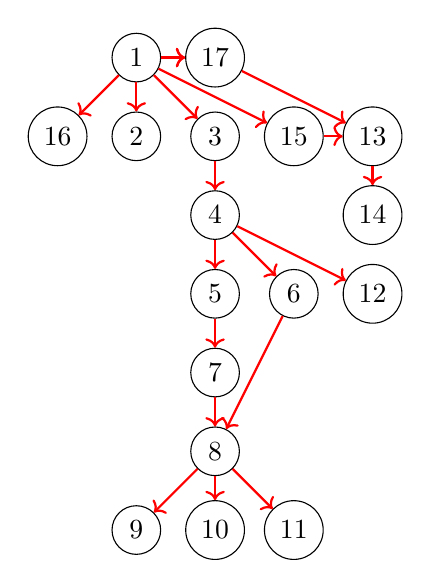
\begin{tikzpicture}
\node[circle, draw] at (0, 0) (1) {1};
\node[circle, draw] at (0, -1) (2) {2};
\node[circle, draw] at (1, -1) (3) {3};
\node[circle, draw] at (1, -2) (4) {4};
\node[circle, draw] at (1, -3) (5) {5};
\node[circle, draw] at (2, -3) (6) {6};
\node[circle, draw] at (1, -4) (7) {7};
\node[circle, draw] at (1, -5) (8) {8};
\node[circle, draw] at (0, -6) (9) {9};
\node[circle, draw] at (1, -6) (10) {10};
\node[circle, draw] at (2, -6) (11) {11};
\node[circle, draw] at (3, -3) (12) {12};
\node[circle, draw] at (3, -1) (13) {13};
\node[circle, draw] at (3, -2) (14) {14};
\node[circle, draw] at (2, -1) (15) {15};
\node[circle, draw] at (-1, -1) (16) {16};
\node[circle, draw] at (1, 0) (17) {17};

\draw[->, Red, thick] (1) to (2);
\draw[->, Red, thick] (1) to (3);
\draw[->, Red, thick] (1) to (15);
\draw[->, Red, thick] (1) to (17);
\draw[->, Red, thick] (1) to (16);
\draw[->, Red, thick] (1) to (17);

\draw[->, Red, thick] (3) to (4);
\draw[->, Red, thick] (4) to (5);
\draw[->, Red, thick] (4) to (6);
\draw[->, Red, thick] (4) to (12);
\draw[->, Red, thick] (5) to (7);
\draw[->, Red, thick] (6) to (8);
\draw[->, Red, thick] (7) to (8);
\draw[->, Red, thick] (8) to (9);
\draw[->, Red, thick] (8) to (10);
\draw[->, Red, thick] (8) to (11);
\draw[->, Red, thick] (13) to (14);
\draw[->, Red, thick] (15) to (13);
\draw[->, Red, thick] (17) to (13);
\end{tikzpicture}
}
\end{center}
\section{Cost of Sanitisation}
In certain cases sanitisation is unavoidable. For example, an object which needs to be clean at the end of the process must be sanitised at least once. However, in certain other cases, sanitisation happens as an unavoidable overhead. Such sanitisation is of the following types:
\begin{enumerate}
\item Sanitising the hand alone.
\item Sanitising a contaminated object which otherwise doesn't need to be sanitised per se (e.g. because it will be eventually disposed), but must be sanitised because it will be part of some action involving other clean objects.
\item Sanitising an otherwise clean object because it came in contact with a contaminated object during the sanitisation routine.
\end{enumerate}

The actual cost of clean/sanitising an object is not uniform across objects. Some are easy to clean (e.g. small items like keys), some are harder (e.g. vegetables), while there are others which are very difficult or practically impossible to clean, e.g. big packets or large clothing items.

\section{Objectives}
The objective of a sanitisation process is to not contaminate any clean object, including our hands. Some of the contaminated objects must be sanitised while some needn't be bothered about. The main objective is to optimise the process in terms of the cost incurred due to sanitisation.

Viewed as a scheduling problem, we want to come up with a schedule $S$, which is nothing but a sequence of actions such that:
\begin{enumerate}
\item All actions are done.
\item All objects required to be clean at the end of the process should indeed be clean.
\item There should be no other schedule $S'$ which has lower cost than $S$.
\end{enumerate}

\section{Scheduling Algorithms}

In this section, we present the various algorithms we design and implement to solve the problem presented in the above sections.

We view the scheduling problem as having the following two components
\begin{enumerate}
\item \emph{Generation of skeletal sequence}, wherein the dependence graph is used to generate a sequence of essential actions.
\item \emph{Introduction of sanitisation}, wherein sanitisation actions are inserted to achieve the scheduling objectives in an optimal way.
\end{enumerate}

\subsection{Generation of skeletal sequence}
The first step is a variant of the well-known topological sort algorithm which runs on the dependency graph and generates a valid total ordering of the essential actions. That algorithm maintains a ready list of actions, i.e. actions which have none of the dependence actions (from the DAG) pending. Out of this ready list the algorithm picks up one which it deems the best to be dispatched next based on a heuristic. This is the step where this algorithm differs from the traditional topological sort algorithm.

\begin{algorithm}
\begin{algorithmic}[0]
\Procedure{skeletan-sequence}{$D : DAG$}
  \State $schedule \gets$ \texttt{[]}
  \State $ready \gets$ $[D.root]$
  \While{$ready \neq $ \texttt{[]}}
    \State $a \gets$ \Call{best-action}{$ready$}
    \State Pop $a$ from $ready$
    \State $dep \gets$ $a.succ$ \Comment{$a.succ$ : the list of $a$'s successors}
    \State Add all elements of $dep$ to $ready$
    \State Add $a$ to $schedule$
  \EndWhile
\EndProcedure
\end{algorithmic}
\end{algorithm}

\section{Introduction of Sanitisation}
\subsection{Branch and Bound Algorithm}

\subsection{Genetic Algorithms}

\section{To Do}
\begin{enumerate}
\item Complexity analysis of the problem
\end{enumerate}
\end{document}